\documentclass{beamer}
\usetheme{CambridgeUS}
\title{Foot classifier}
\subtitle{Progetto IC}
\author{Luigi Lomasto, Marco Mecchia}
\date{29 Febbraio 2016}
\usepackage[italian]{babel}
\usepackage[latin1]{inputenc}
\usepackage[T1]{fontenc}
\usepackage{graphicx}
\usepackage{pgf}
\usepackage{multimedia}
\usepackage{listings}
\usepackage{amsmath}

\begin{document}
	\begin{frame}
		\maketitle
		Prof. Roberto Tagliaferri \newline
		
		Dott. Michele Fratello\newline
		Dott. Paola Galdi \newline
		Dott. Angela Serra
		
	\end{frame}
	
\begin{frame}
	\frametitle{Outline}
	\tableofcontents
\end{frame}

\section{Introduzione al problema}

\begin{frame}
	\frametitle{Il problema}
	Dato un insieme di immagini piedebarometriche, classificare automaticamente le seguenti patologie:
	\newline
	 \begin{itemize}
	\item Cavo
	\item Piatto
	\item Normale
	\item Valgo
    \end{itemize}
\end{frame}

\begin{frame}
	\frametitle{Patologie}
	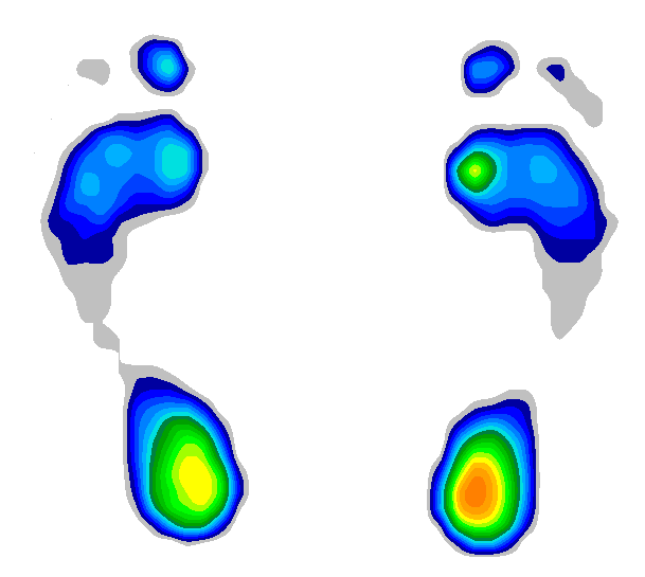
\includegraphics[keepaspectratio,height=95px]{immagini/0_cleared.png}
	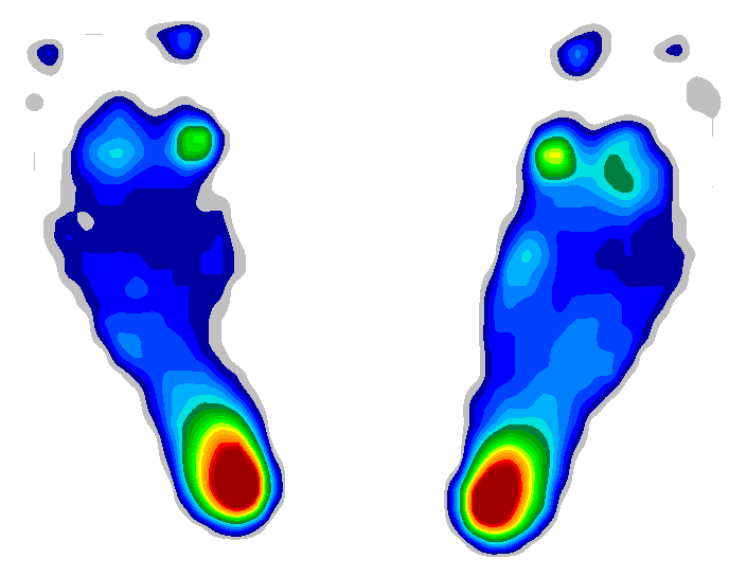
\includegraphics[keepaspectratio,height=95px]{immagini/1_cleared.png}
	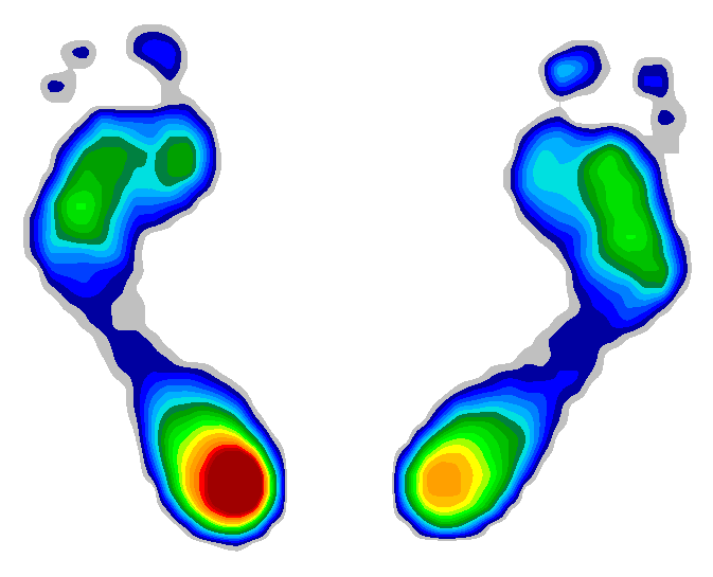
\includegraphics[keepaspectratio,height=95px]{immagini/2_cleared.png}
\end{frame}

\section{Dataset}
\begin{frame}
	\frametitle{Struttura del dataset}
	Il dataset � costituito da 190 piedi (95 coppie) di cui:
	\begin{itemize}
		\item 121 Cavi
		\item 13 Piatti
		\item 56 Normali
	\end{itemize}
	per la prima classe di patologie, mentre:
	\begin{itemize}
		\item 88 Valghi
		\item 102 Normali
	\end{itemize}
	per la seconda classe di patologie.
\end{frame}

\section{Preprocessing}
\begin{frame}
	\frametitle{Panoramica}
	Nella fase di preprocessing, abbiamo eseguito le seguenti operazioni.
	\begin{itemize}
		\item Conversione delle immagini .bmp in .png.
		\item Pulizia delle immagini (rimozione del baricentro).
		\item Trasformazione delle immagini in scala di grigio.
		\item Divisione, rotazione e cropping dei piedi.
	\end{itemize}
	\centering
\end{frame}

\subsection{Trasformazione delle immagini}

\begin{frame}
	\frametitle{Trasformazione delle immagini}
	\begin{itemize}
		\item Trasformazione da uno spazio 3D (R,G,B) ad uno spazio 1D.
		\item Necessaria per valutare la pressione in un pixel dell'immagine.
		\item Problema: Come associare ad ogni tripla (R,G,B) il valore di intensit\'a corretto?
	\end{itemize}
\end{frame}

\begin{frame}
	\frametitle{Prima soluzione}
	\begin{itemize}
		\item Clustering sulle immagini.
		\item Trovati i centroidi, sostituire ogni pixel dell'immagine con il rappresentante del proprio cluster.
		\item Ordinare i centroidi per intensit\'a crescente e associare valori compresi tra 0 e 1.
		\item Problemi: Trovare il k adatto, trovare un ordinamento per i cluster.
	\end{itemize}
\end{frame}

\begin{frame}
	\frametitle{Soluzione definitiva}
	\begin{itemize}
		\item Variante della prima soluzione.
		\item Possibile grazie alla scala colorata delle pressioni fornita dal medico.
	\end{itemize}
	\begin{center}
		
\includegraphics[keepaspectratio,width=300px]{immagini/color.png}
	\end{center}
\end{frame}

\subsection{Divisione, rotazione e cropping delle immagini}

\begin{frame}
	\frametitle{Rotazione e cropping delle immagini}	
	\begin{itemize}
		\item La divisione \'e stata necessaria per separare piede destro da piede sinistro.
		\item La rotazione non \'e strettamente necessaria.
		\item Il cropping rimuove la parte di sfondo superflua.
	\end{itemize}
\end{frame}

\begin{frame}
	\frametitle{Rotazione del piede}
	Per ruotare il piede abbiamo utilizzato un algoritmo molto semplice:
	\begin{enumerate}
		\item Abbiamo trovato il centro
	\end{enumerate}
\end{frame}

\section{Features extraction}
\begin{frame}
	\frametitle{Features extraction}
	Terminata la fase di preprocessing siamo passati alla fase di features exstraction. Nel nostro caso, le regioni d'interesse di ogni piede differiscono significativamente tra loro. Per questo motivo, � stato necessario implementare algoritmi ad-hoc per l'estrazione delle features. 
	\newline
	Dovendo lavorare con due classi di patologie:
	\begin{itemize} 
		\item Cavo, piatto e normale.
		\item Valgo e normale.
    \end{itemize} 
   
   sono stati implementati due algoritmi per l'estrazione delle features.
\end{frame}

\subsection{Features primo classificatore}
\begin{frame}
	\frametitle{Features primo classificatore (1/2)}
	Le features estratte per le patologie appartenenti alla prima classe sono le seguenti:
	\begin{itemize}
		\item \textbf{lengthMinIstmo:} esprime la lunghezza minima che assume l'istmo.
		\item \textbf{lengthMediaIstmo:} esprime la lunghezza media dell'istmo.
		\item \textbf{lengthMaxAvampiede:} esprime la massima lunghezza che assume l'avampiede.
		\item \textbf{indexPathology:} Si ottiene dal rapporto $\frac{lengthMaxAvampiede}{lengthMinIstmo}$
		\item \textbf{mediumPressure:} Indica la pressione media esercitata dal piede.
	\end{itemize}
	
\end{frame}
\begin{frame}
	\frametitle{Features primo classificatore (2/2)}
    \centering
     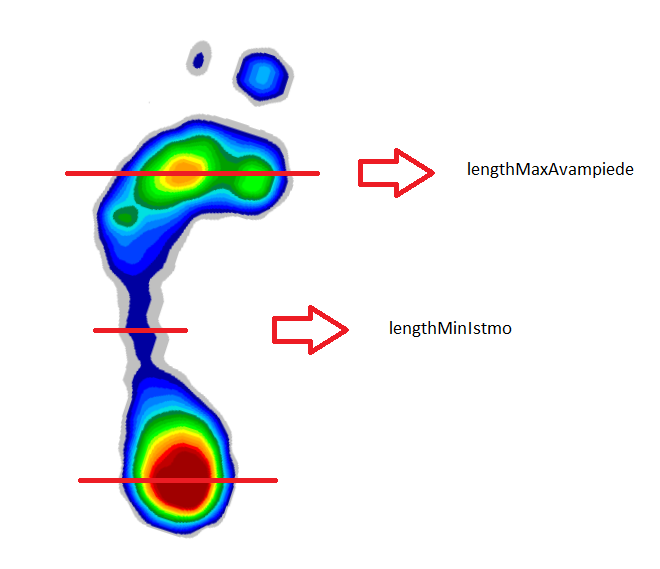
\includegraphics[keepaspectratio,height=220px]{immagini/Immagine.png}
\end{frame}

\subsection{Features secondo classificatore}
\begin{frame}
	\frametitle{Features secondo classificatore (1/2)}
	Le features estratte per le patologie appartenenti alla seconda classe sono le seguenti:
	\begin{itemize}
		\item juve
		\item juve
	\end{itemize}
	
\end{frame}
\begin{frame}
	\frametitle{Features secondo classificatore (2/2)}
immagine
	
\end{frame}
\section{Features Selection}
\begin{frame}
	\frametitle{Features Selection}
	La features selection � stata fatta in modo esaustivo. 
	\newline
	\newline
	\newline
	Motivi:
	\begin{itemize}
		\item Basso numero di features usate.
		\item Si valutano tutti i possibili sottoinsiemi di features.
		\newline
	\end{itemize}
	Sottoinsiemi valutati:
	\begin{itemize}
		\item 31 per il primo classificatore.
		\item 15 per il secondo classificatore.
	\end{itemize}
	
\end{frame}
\section{Infrastruttura}
\begin{frame}
	\frametitle{Infrastruttura}
	  L'infrastruttura software � la seguente:
	  	\begin{itemize}
	  		\item $ \forall $ Sottoinsieme di features
	  		\begin{itemize}
	  			\item Per N volte
	  			\begin{itemize}
	  				\item Dividiamo il dataset in train e test
	  				\item Cross Validation sul train per stimare la configurazione migliore.
	  				\item Calcolo delle accuratezze sul test.
	  			\end{itemize}
	  			\item Calcolo delle accuratezze medie.
	  		\end{itemize}
	  	\end{itemize}
	  	
	  	Il sottoinsieme scelto � quello con accuratezza totale media  pi� alta.
	  
\end{frame}
\section{Scelta dei classificatori}

\begin{frame}
	\frametitle{SVM Gaussiano (Radial-Basis-Function) (1/2)}
  Classificatore usato: \textbf{SVM Gaussiano (Radial-Basis-Function)}.\newline \newline
  Scelta dovuta ai seguenti motivi :
  	\begin{itemize}
  		\item RBF ben di adatta a problemi di classificazione dove il dataset � significativamente pi� grande rispetto al numero di dimensioni.
  		\item Reti Neurali troppo complesse per il problema affrontato.
  		\item SVM lineare generalmente usato quando si ha alta dimensionalit�. 
  	\end{itemize}
	
\end{frame}

\begin{frame}
	\frametitle{SVM Gaussiano (Radial-Basis-Function) (2/2)}
	L' RBF � uno dei kernel pi� popolari. Esso aggiunge un "bump" attorno a ciascun punto di dati. \newline  \newline
    E' espresso come: $ f(x)= \sum\limits_{i=1}^m \alpha_{i} exp(-\gamma \(|| x_{i} - x ||\)^{2}) + b $ 
  
	
\end{frame}
	

\section{Risultati}
\section{Conclusioni}

\end{document}
